\section{Additional empirical results}
\label{sec:extra-additional-results}
In this section we provide some additional results about our debiasing technique, mainly focusing on the worst-case scenarios described in Section~\ref{sec:analysis-mnist}. 


\begin{table}
    \centering
    \begin{tabular}{c c c}
         \toprule
         $\rho$ & Vanilla & EnD  \\
         \midrule
         0.1 & 99.21 & 99.24\std{0.05} \\
         \bottomrule 
    \end{tabular}
    \caption{Debiasing on an unbiased training set ($\rho=0.1$)}
    \label{table:mnist-unbiased-training}
\end{table}

\begin{table}
    \centering
    \begin{tabular}{c c c c}
        \toprule
        $\rho$ & Vanilla &  EnD (target) & EnD (random) \\
        \midrule
        0.995 & 72.10\std{1.90} & 72.25\std{0.56}  & 66.68\std{0.35} \\
        \bottomrule
    \end{tabular}
    \caption{Debiasing on incorrect bias labels. Target means that target labels are also used as bias label (i.e. $t_i = b_i$, worst case), random means that bias labels are assigned randomly.}
    \label{table:mnist-wrong-pseudo}
\end{table}

\subsection{Debiasing on an unbiased dataset}
\label{extra:debias-on-unbiased}

Here we show that the supervised EnD regularization does not deteriorate the final results if applied on a training set which is not biased. Table~\ref{table:mnist-unbiased-training} shows the results of training with EnD on Biased-MNIST with $\rho=0.1$.
In this setting, applying the regularization term is not harmful for obtaining good generalization: this is because in a supervised setting we still have access to the correct color labels, thus we do not perform disentanglement over any useful features for the network.
This is a trivial result, however with this demonstrated we can now focus on an unbiased training set in the unsupervised case.

\subsection{Debiasing with wrong pseudo-labels}
\label{extra:debias-on-wrong-bias}


\begin{figure}
    \centering
    \begin{subfigure}{0.8\columnwidth}
        \centering
        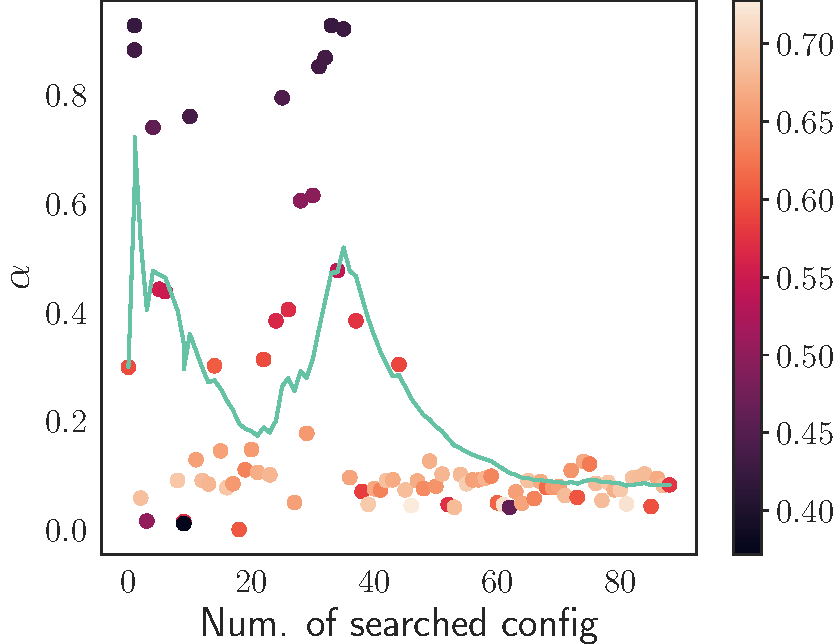
\includegraphics[width=1\columnwidth]{appendix/img/alpha_time.pdf}
        \caption{~}
        \label{fig:alpha-vs-time}
    \end{subfigure}\\[1em]
    \begin{subfigure}{0.8\columnwidth}
        \centering
        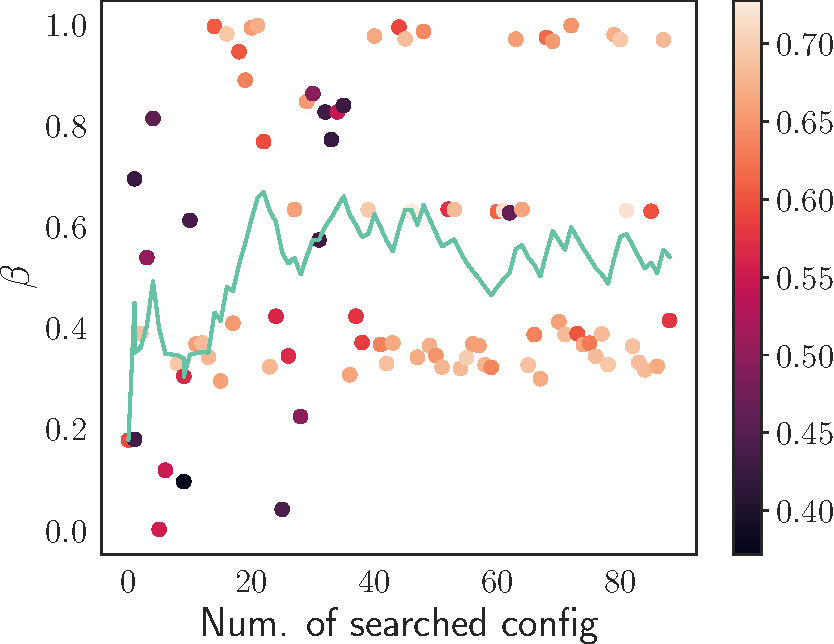
\includegraphics[width=1\columnwidth]{appendix/img/beta_time.pdf}
        \caption{~}
        \label{fig:beta-vs-time}
    \end{subfigure}

    \caption{{Evolution of (a) $\alpha$ and (b) $\beta$ versus the number of searched configs} during the hyperparameters optimization with incorrect pseudo-labels. We can observe how the optization process drives $\alpha$ towards 0, while $\beta$ does not seem to be revelant. The point color indicates the accuracy on the unbiased test set, while the line shows the trend as an exponetially weighted moving average computed with a smoothing factor of $0.1$.}
    \label{fig:alpha-beta-vs-time}
\end{figure}

We now assume that the pseudo-labels we compute are not representative of the true bias attributes. 
Using Biased-MNIST as case study, we identify that the worst-case scenario for the pseudo-labeling step corresponds to using a completely unbiased dataset (i.e. $\rho=0.1$) for training the biased encoder.
Taking into account the results shown in Section~\ref{extra:debias-on-unbiased}, performing the pseudo-labeling step in this setting this will most likely result in pseudo-labels corresponding to the actual target class rather then the background color.
We emulate this event by setting the bias label $b_i$ equal to the target label $t_i$ for every sample in the dataset, and then we the apply EnD algorithm. 
To test this worst-case with EnD, we choose $\rho=0.995$ as it provides a way for the final accuracy to both a decrease or increase with respect to a vanilla model. 
The results are reported in Table~\ref{table:mnist-wrong-pseudo}, and noted as \emph{target}. Even in this case, we are able to retain the baseline performances, altough we do not obtain any significant improvement. 
This is thanks to the hyperparameter optimization policy that we employ (recall that we assume an unbiased validation set - even if small - is available). 
Figure~\ref{fig:alpha-beta-vs-time} visualizes the evolution of the hyperparameters $\alpha$ and $\beta$ while searching for possibile configurations. 
In this setting, $\alpha$ represents the most dangerous term, as it enforces decorrelation among samples with the same class, conflicting with the cross-entropy term. 
However, the optimization process drivers $\alpha$ towards 0, making it effectively non-influent on the loss term. 
On the other hand, the entangling term $\beta$ does not bring any contribution to the learning process: it is, in fact, useless as there is full alignment between target and bias labels, hence $B(i)$ = \O. 
A possible scenario in which $\beta$ would not have null influence, is if we do not impose $t_i = b_i$. 
We explore the extreme setting by assigning a random value to $b_i$ for every sample $i$. The results are reported as \emph{random} in Table~\ref{table:mnist-wrong-pseudo}. In this case it is possible to observe a drop in performance with respect to the baseline. However, we argue that random pseudo-labels would be the result of poor representations due to possibly underfitting models or lack of sufficient training data - which, in a practical setting, would be a more pressing issue. 